\section{Projektstyring}
\subsection{Scrum}
Vi har anvendt \textit{Scrum} som værktøj til projektstyring igennem hele forløbet med hovedopgave.
Det gav os nogle gode retningslinjer for hvordan vi har skulle planlægge projekt, samtidig med at det har givet mulighed for nemmere at forhindre at vores projekt gik i den forkerte retning.
I forlængelse af at vi typisk har villet prøve at undgå fejl eller dårligere perioder samt dårlig arbejdsgang, gav Scrum os mulighed for
at rette op på de ting der gik skidt eller hvis vi var utilfreds med noget.

\subsection{Planlægning}
Vi har anvendt Scrum til at planlægge vores sprints.
\\
Hvert sprint har varet 2 uger, hvoraf den første dag var sat af til planlægning at opgaver og prioritering af disse.
Den sidste dag i sprintet har ligeså været afsat, her har vi afholdt review og retrospective.
\\
Vi har på den måde fået samlet op på sprintet og snakket om hvordan de sidste par uger er gået, på godt og ondt.
\\\\
Ved at bruge Scrum, har vi hele tiden sørget for at holde os på rette spor, og lave de mest relevante opgaver.
Der var f.eks. efter første sprint, et behov for at ændre i vores opgaver, da vi havde brugt vores tid på irrelevante funktioner i systemet.
Ved at få feedback, kunne vi ændre retning og begynde på havde mere relevans for systemet og vores interessenter.
\\\\
Vi har også haft mulighed for at ændre på mere personlige ting, eller hvis der har været nogle udfordringer der krævede opmærksomhed.
\\
Det kunne forekomme at man havde en stresset periode på hjemmefronten, og derfor ikke ville arbejde så fokuseret i en periode.
Denne arbejdsmetode gav os mulighed for at justere opgavernes omfang, alt efter hvor meget eller lidt vi kunne arbejde.
\\\\
Brugen af Scrum har fungeret efter hensigten og har været en stor hjælp, da vi har haft en rettesnor til planlægningen af projektet.
\\\\
Ved hvert retrospective har vi hver skrevet et tal fra 1-5, hvor 1 er lavest og 5 er højest. Dette tal summerer op hvor godt vi personligt
har haft det i løbet af sprintet.
Til tallet følger det nogle positive og negative kommentarer, som har været en forklaring på det tal hver person er endt på.
Vi har herefter talt frit fra leveren om de gode og dårlige oplevelser der har været i løbet af sprintet, og så har scrum masteren sørget for at
eventuelt dårlige oplevelser er blevet løst.
\\\\
Vi har tilføjet en graf der viser det gennemsnitlige humør-tal uge for uge.
\\
Den afspejler hvor godt gruppen synes forløbet er gået.
\\\\
\begin{figure}[here]
    \makebox{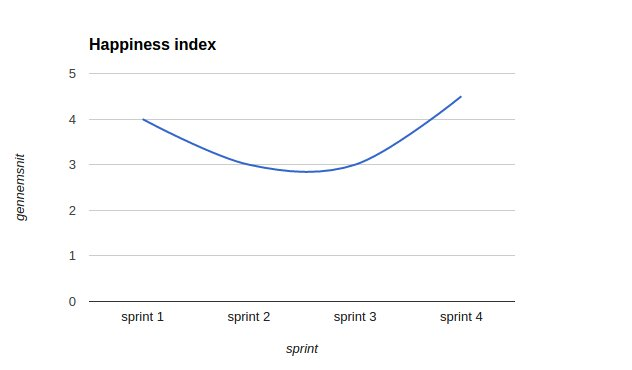
\includegraphics[scale=0.75]{Happiness_graf}}
    \caption{Graf der viser vores happiness index i vores sprints}
    \label{fig:happiness-graf}
\end{figure}

Forklaringen på grafen er at vi var meget positive efter første sprint, hvor vi havde lavet analyse og forberedelser.
Vi skulle til at kode systemets første funktioner og klasser, og vi var derfor meget fortrøstningsfulde.
\\
Desværre gik det ikke helt som forventet, da vi fik negativ feedback og blev nødt til at ændre vores planlægning og prioritering,
og vi blev nærmest nødt til at starte forfra, hvilket også ses midt på grafen.
\\
Vi endte dog med et fornuftigt produkt, og overholdt vores sidste deadline. Efter sidste sprint fik vi meget konstruktiv feedback, 
som kan blive afgørende for produktets videreudvikling og vi kunne også bruge noget af det til personlig udvikling.

\subsection{Scrum værktøjet YouTrack}
I projektperioden har vi anvendt YouTrack til at visualisere metoder fra Scrum.
\\
Selvom vi har anvendt andre værktøjer på studiet og i praktikken, faldt valget på YouTrack, da dette værktøj er gratis og
har givet os nødvendig funktionalitet, for at kunne planlægge opgaver og holde styr på deres stadier.
\\\\
YouTrack giver mulighed for at lave rapporter, hvor vi kun har brugt muligheden for at lave et burndown chart. Herudover kan man oprette
en backlog og et sprint. Herefter har man mulighed for at opdele sine backlog opgaver og trække dem ud i en såkaldt \textit{swim lane}, der har forskellige
stadier, \textit{Open}, \textit{In Progress}, \textit{Fixed}, \textit{Verified}. På denne måde kan vi hele tiden opdatere hvor langt i processen vi er nået
med de enkelte opgaver, og få et overblik over hvad medlemmerne i gruppen laver eller hvad der mangler at blive lavet i det nuværende sprint.
\\
En mangel i Youtrack har været at vi ikke har haft mulighed for at lave en projekt backlog. Denne bruges typisk til at indeholde de overordnede opgaver i
projektet som mangler at blive lavet. Da vi følte det nødvendigt at have en sådan backlog, har vi selv valgt at lave et dokument på Google Docs, og gjort det tilgængeligt
for begge gruppens medlemmer. Dette dokument bruges til at skabe et overblik over hvilke overordnede opgaver vi har tilbage i projektet, samt tilføje nye opgaver der kan opstå.
Listen er delt op i opgaver til det konkrete system og vores rapport, og hver gang vi har skulle planlægge nye sprints, har vi taget opgaver fra vores projekt backlog over i
det enkelte sprints backlog.
\\\\
Vi har nedenfor tilføjet nogle reelle eksempler fra vores projektperiode, af et burndown chart, en swim lane med opdelte opgaver fra backlog'en og vores projekt backlog.
\begin{figure}[here]
    \makebox{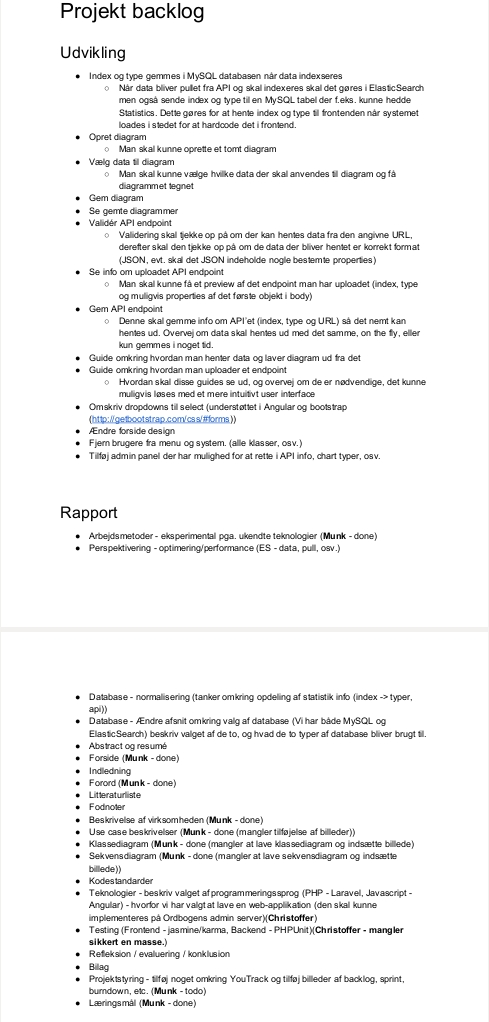
\includegraphics[scale=0.75]{Projekt_backlog}}
    \caption{Vores projekt backlog dokument}
    \label{fig:projekt-backlog}
\end{figure}
\begin{figure}[here]
    \makebox[\textwidth]{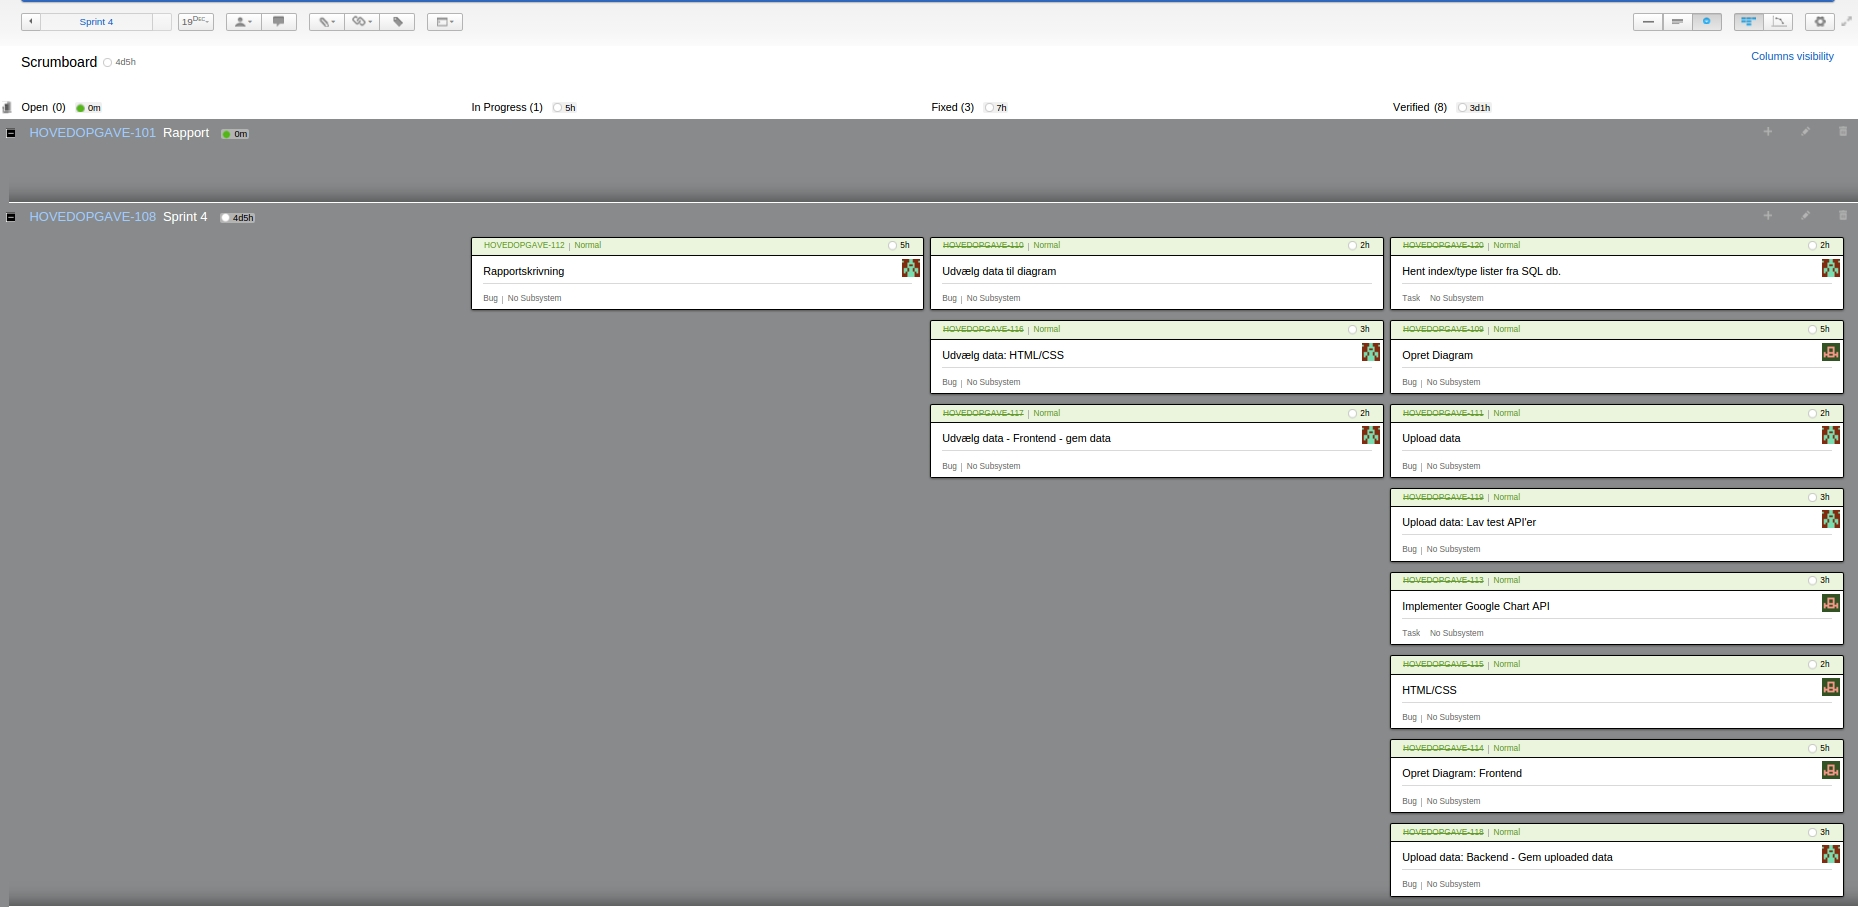
\includegraphics[scale=0.45]{Swim_lane}}
    \caption{Swim lane fra sprint 4}
    \label{fig:swim-lane}
\end{figure}
\begin{figure}[here]
    \makebox[\textwidth]{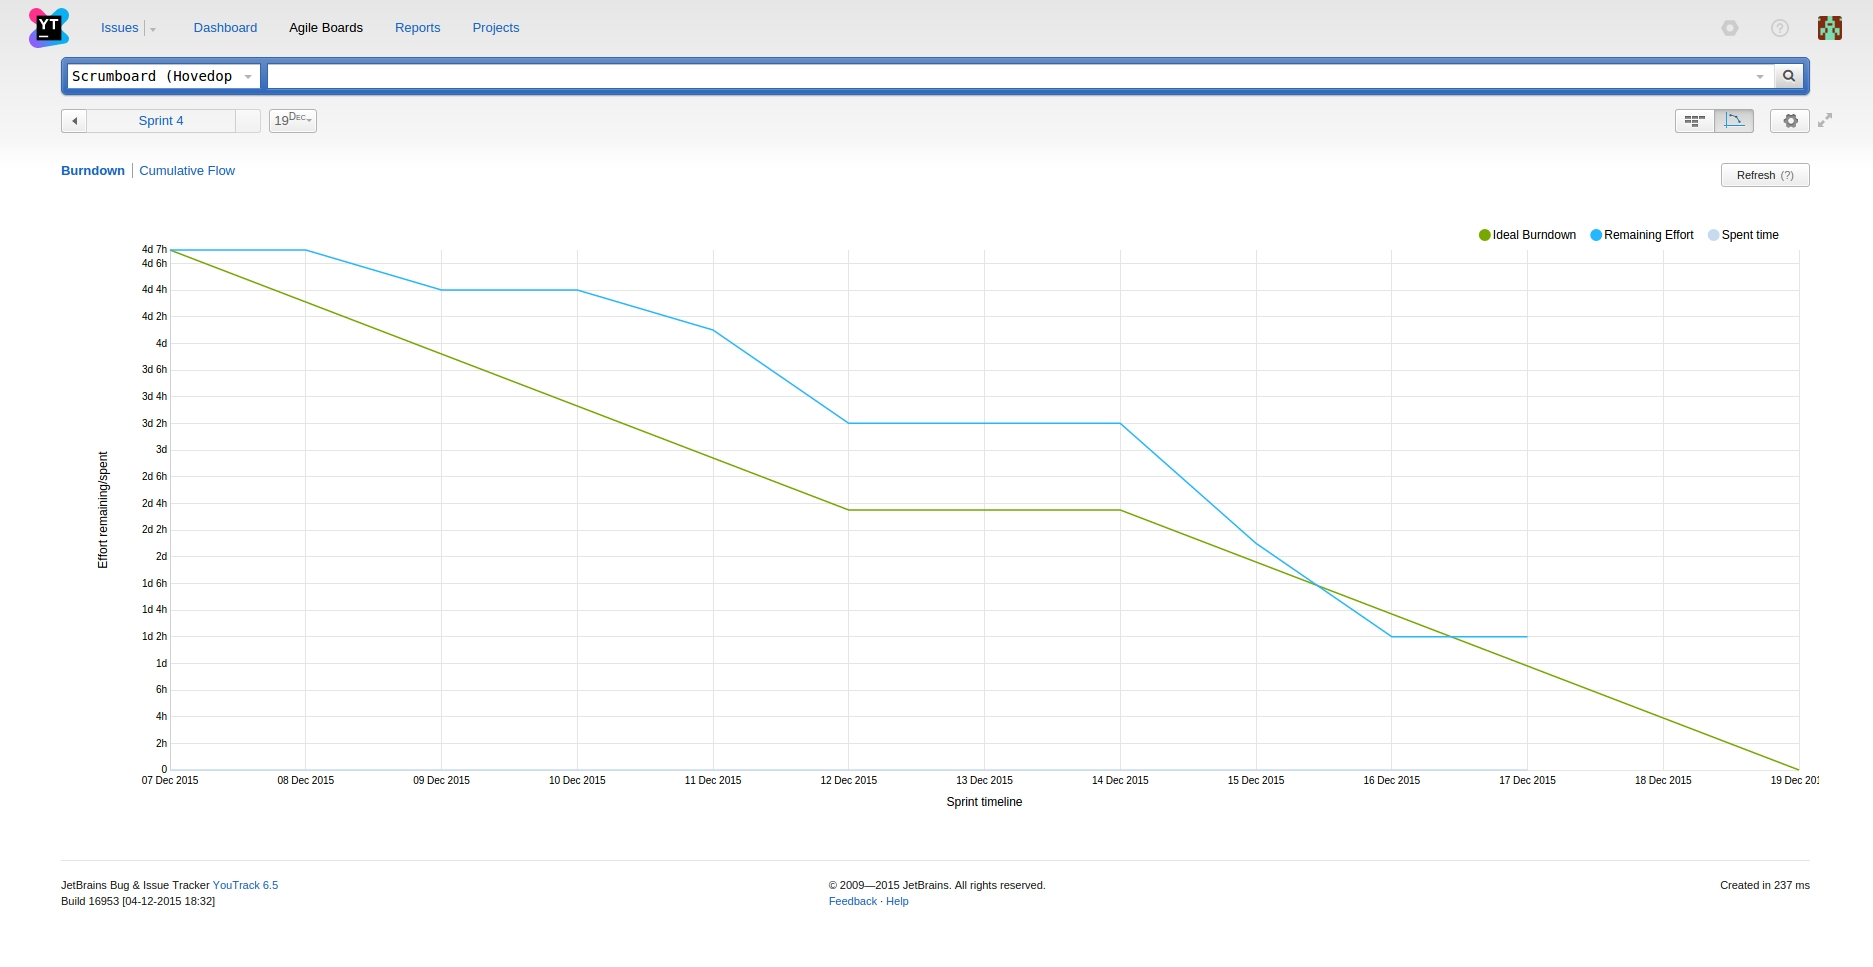
\includegraphics[scale=0.35]{Burndown_chart}}
    \caption{Burndown chart fra sprint 4}
    \label{fig:burndown-chart}
\end{figure}
\subsection{Review referater}
I dette afsnit vil vi referere de vigtigste ting fra sprint reviews i løbet af projektperioden
\subsubsection{Fredag d. 20/11}
Tilstedeværende til mødet: Mikkel, Christoffer, Michael og Peter.
\\\\
Vi præsenterede hvad vi havde lavet i løbet af sprintet, som primært var CRUD til håndtering af brugere. Derudover havde vi brugt meget tid på at strukturere systemet, skrive rapport, generel opsætning af teknologier, mm.
Det feedback vi fik var at vi skulle fokusere mere på at lave kernefunktionalitet til systemet, så de funktioner der var vigtige for interessenter skulle vi fokusere på i stedet for f.eks. et brugersystem.
Derudover fik nogle fingerprej om hvilken retning vi skulle gå i med projektet og hvad der var vigtigt for systemet.
Nogle punkter vi kunne tage med var,
\begin{itemize}
    \item{Pull eller push af data?}
    \item{Fokus på funktionalitet}
    \item{Vælg en sti og gør den færdig (et diagram ad gangen)}
    \item{Kig evt. på google analytics mht. hentning af data (api keys)}
    \item{Guide til upload/hentning af data}
\end{itemize}
\subsubsection{Fredag d. 4/12}
Tilstedeværende til mødet: Mikkel, Christoffer, Michael og Peter.
\\\\
Vi præsenterede hvad vi havde lavet i løbet af sprintet, som var hentning og visning af data, upload af API endpoint. Derudover fortalte vi omkring vores research mht. ElasticSearch og hvordan vi havde valgt at vi vil pulle vores data fra API'er frem for at det bliver pushet til vores server. På denne måde kan vi nemmere kontrollere hvad og hvor meget data der er tilgængeligt på vores ElasticSearch server.
Det feedback vi fik var at vi skulle gøre det mere specifikt hvad der skulle uploades, så det ikke er rå data der bliver uploadet til vores server, som vi skal behandle og lave statistik data ud fra, det skal være ren statistik data der bliver uploadet. På den måde skaber det mere arbejde for dem der skal uploade, men det gør at vi kun har ren statistik tilgængelig på vores server. Dette giver ikke så mange plads problemer, da det ikke fylder specielt meget at have en dato og et tal, i forhold til en masse objekter osv. Det er primært en dato eller et tidspunkt der skal være en parameter, og så en parameter der angiver et tal eller lignende for det tidspunkt.
Derudover fik vi lidt feedback på hent og vis data, i forhold til hvordan det skal fungere når der skal laves diagrammer.
Generelt gik det meget bedre end først review, og vi var på rette vej i forhold til et mere fuldendt produkt. Generelt skal vi fokusere mere på at fortsætte i samme retning, men med små-justeringer. På denne måde kan vi virkelig få gavn af disse reviews og få noget løbende feedback fra vores interessenter.
\subsubsection{Fredag d. 18/12}
Tilstedeværende til mødet: Mikkel, Michael og Peter.
\\\\
Mikkel præsenterede hvad vi havde lavet i løbet af sprintet, som var Upload af API endpoint, en del af valideringen af API, Gem API data, dynamisk hentning af index/type lister og oprettelse af et diagram.\\
Herudover var der også en demo, hvor der blev gennemgået alle funktioner samt fejlhåndtering i systemet. Grunden til dette, var at vi på dette tidspunkt har lavet alle de grundlæggende funktioner til at løse
problemstillingen, og vi synes det var tid til at få et overblik.\\
Det feedback vi fik, var at det var rart at se hele flow'et fungere, og at vi kunne få vist noget data i forskellige diagramtyper. (Cirkeldiagram, søjlediagrammer og graf).\\
Dog synes de at vi skal ændre i API strukturen, og den måde det bliver hentet og vist på.
De kunne godt tænke sig at man henter fra et bestemt API, som er bestående af et datasæt der indeholder et timestamp og en værdi. Ved hjælp af denne data skal systemet så kunne
udregne statistik data på årlig, månedlig og daglig basis.\\
Man skal så have mulighed for at vælge enten år, måned eller dag samt et tidsinterval man gerne vil have at ens graf skal repræsentere.\\
Derudover skal det være muligt at lave flere grafer i samme diagram, så det er muligt at sammenligne forskellige datasæt.\\\\
Det var rigtig rart at kunne vise alle funktionerne i programmet samtidig, og få feedback på det samlede system. Interessenterne var derudover generelt glade for produktet, og viste en iver og et
ønske for at tilføje og ændre i funktionerne til systemet, hvilket bare er fedt at de er så engagerede omkring ens produkt. Dette giver noget ekstra blod på tanden til at færdiggøre og skabe et værdifuldt
produkt.
